\section{Mission}
\subsection{Choix des technologies}

\subsubsection*{Flutter}
\addcontentsline{toc}{subsubsection}{Flutter}


Pour réaliser la POC, nous avons décidé d'utiliser le framework Flutter de Google\cite{Flutter}. Ce framework permet le développement d'applications cross plate-formes natives\footnote{sur Android, IOS, Web, Linux, Windows et Mac}.

\begin{figure}[h!]
    \centering
    
\includegraphics[scale=0.5]{img/Flutter.jpg}
    \caption{Flutter, un framework Google cross-plateforme}
    \label{fig:Flutter logo}
\end{figure}

Bien que décrié par certain comme une simple tendance ou un framework non-viable sur le long terme, Flutter s'est pourtant hissé à la première place en terme de framework cross-plateforme avec 45\% de votes\footnote{D'après une étude menée par SlashData\cite{Flutter2.2}}. Des entreprises telle que \textbf{BMW}, \textbf{Tencent} (avec son application WeChat utilisée par 1.2 Milliards d'utilisateurs), ou encore \textbf{Toyota} \footnote{Flutter sera au cœur du système d'infotaienment de la prochaine génération de véhicules.} l'utilisent ; même des projets open-source de grande ampleur comme \textbf{Ubuntu} s'y sont mis \footnote{la totalité de l'installer a été redesigné en Flutter\cite{UbuntuFlutter}}.\\

\begin{figure}[!h]
    \centering
    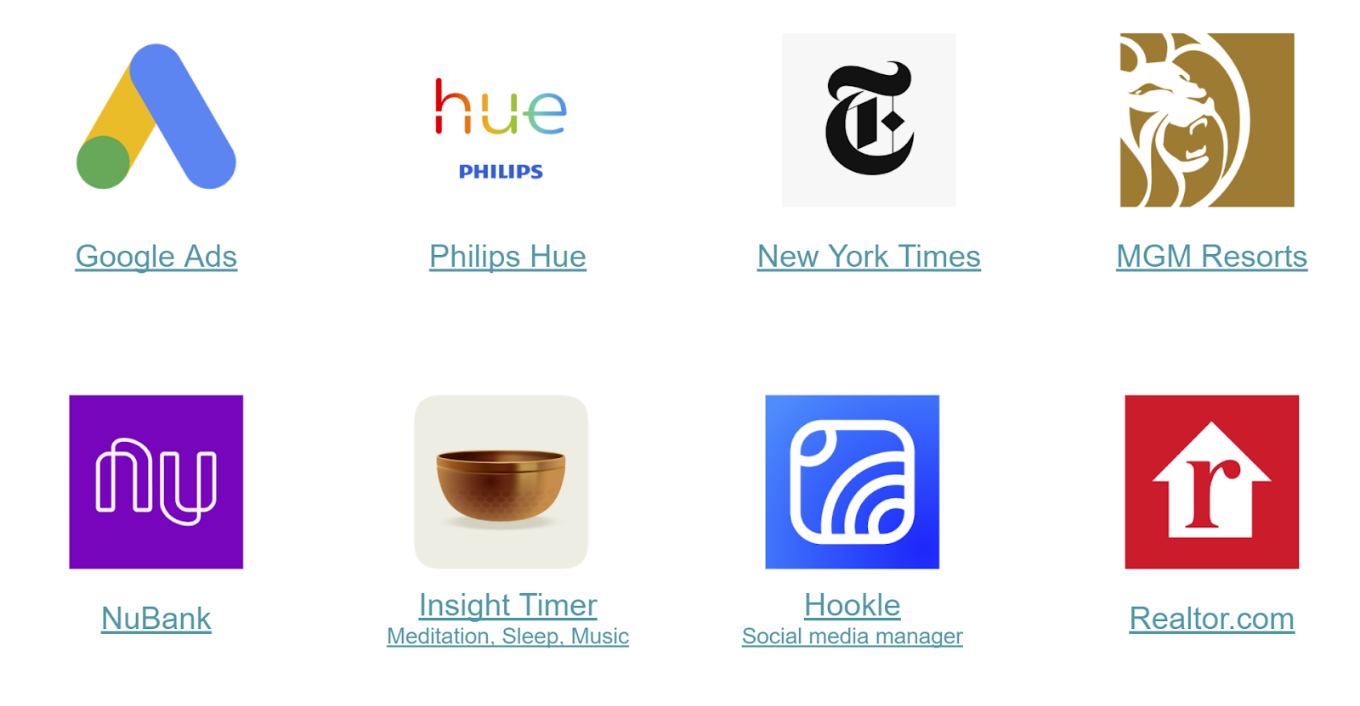
\includegraphics[scale=0.33]{img/Apps_flutter.png}
    \caption{Quelques applications codées à l'aide de Flutter}
    \label{fig:my_label}
\end{figure}

Flutter est très orienté design responsive, les interfaces créées avec s'adaptent donc à toutes les tailles d'écran. De par sa compatibilité avec les smartphones, Flutter propose de nombreux packages utilisables par tactile, il s'imposait comme une technologie de choix pour nous.\\
De plus, notre team de développeurs était déjà formé à cette technologie et avait déjà réalisé plusieurs projets avec ce framework, que ce soit en cours ou en entreprise.\\

Depuis sa version 2.0 sortie début mars 2021, Flutter supporte le développement Web depuis sa branche \texttt{stable}. Il est même proposé aux utilisateurs de télécharger la web app sur leur appareil lorsqu'ils se rendent sur le site.\\
Nous avons donc concentré nos efforts sur cette plateforme, mais une application mobile peut être une piste pour le projet final.

\subsubsection*{Firebase}
\addcontentsline{toc}{subsubsection}{Firebase}

Pour ce qui est du stockage des données, nous avons porté notre choix sur \textbf{Firebase}, la solution de base de données \textbf{NoSQL}\footnote{“Non-SQL" ; les bases de données NoSQL sont, à l'inverse des bases de données SQL, non-structurées, d'où leur nom.}\cite{NoSQL} de Google\cite{Firebase}. Comme Flutter et Firebase sont deux technologies de Google, il est donc très facile de les coupler. Cette plateforme est gratuite en dessous des 10 k écriture/lectures par mois, ce qui est très largement suffisant pour une POC.\\

\begin{figure}[h!]
    \centering

\includegraphics[scale=0.15]{img/firebase.png}
    \caption{Firebase, la solution de base de données NoSQL Google}
    \label{fig:Firebase Logo}
\end{figure}

D'après notre expérience en développement, la forte disponibilité de cette solution en fait l'outil parfait pour une application professionnelle. En effet, comme la totalité de la base de données est hébergée par Google, Panorama Performance n'aura pas à se soucier de la sécurité des données (redondance, sauvegarde, cryptage), ni de la gestion d'un serveur (maintenance, scalabilité horizontale et verticale, \dots).\\

\begin{figure}[!h]
    \centering
    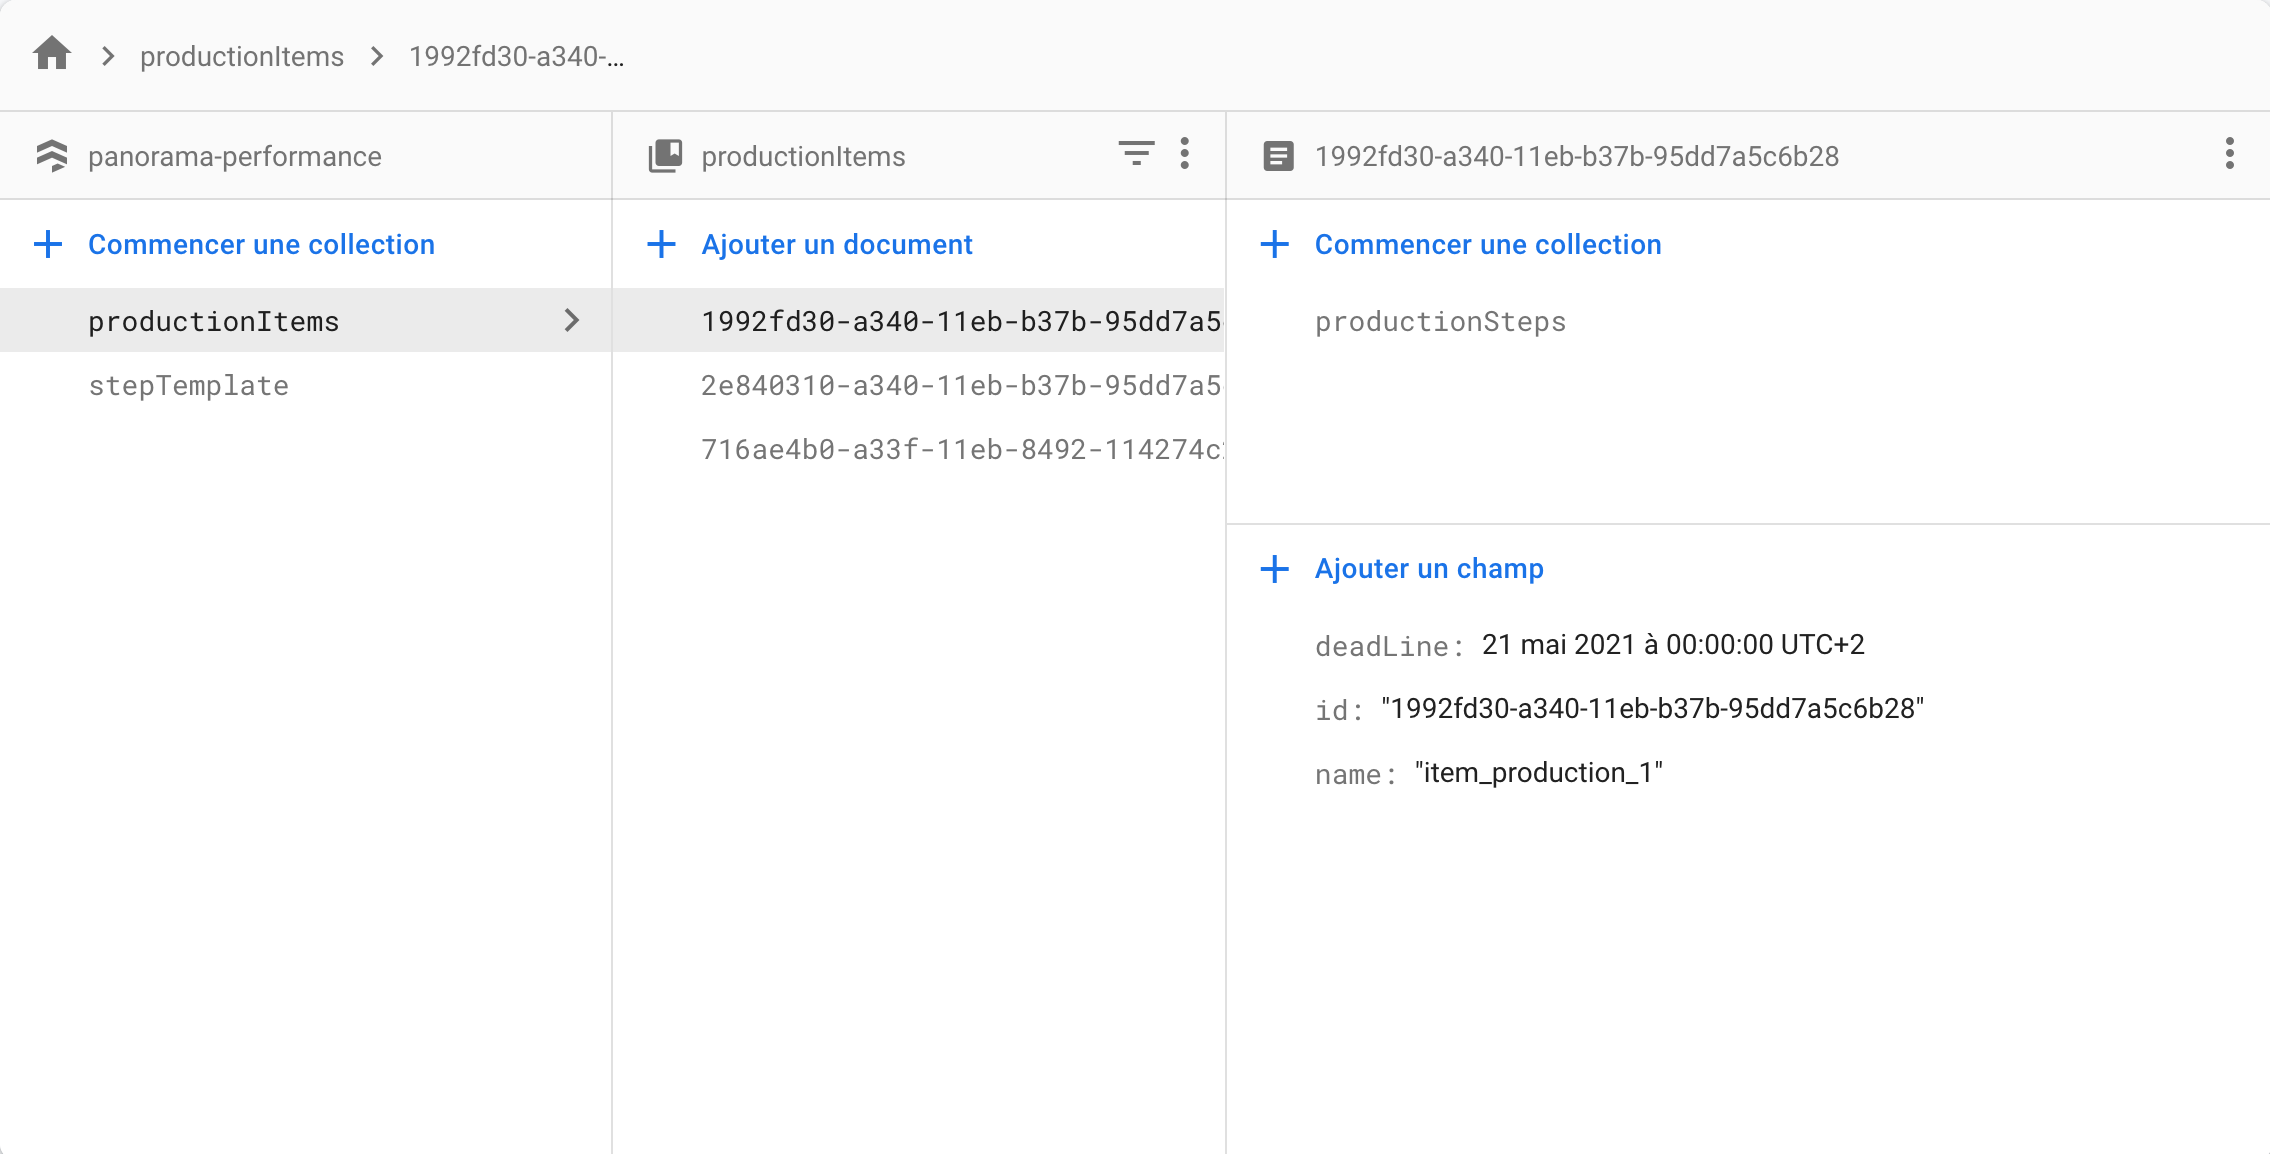
\includegraphics[scale=0.2]{img/screen_firebase.png}
    \caption{Capture d'écran de la base de données NoSQL au 20 mai 2021}
    \label{fig:CaptureFirebase}
\end{figure}

\begin{figure}[!h]
    \centering
    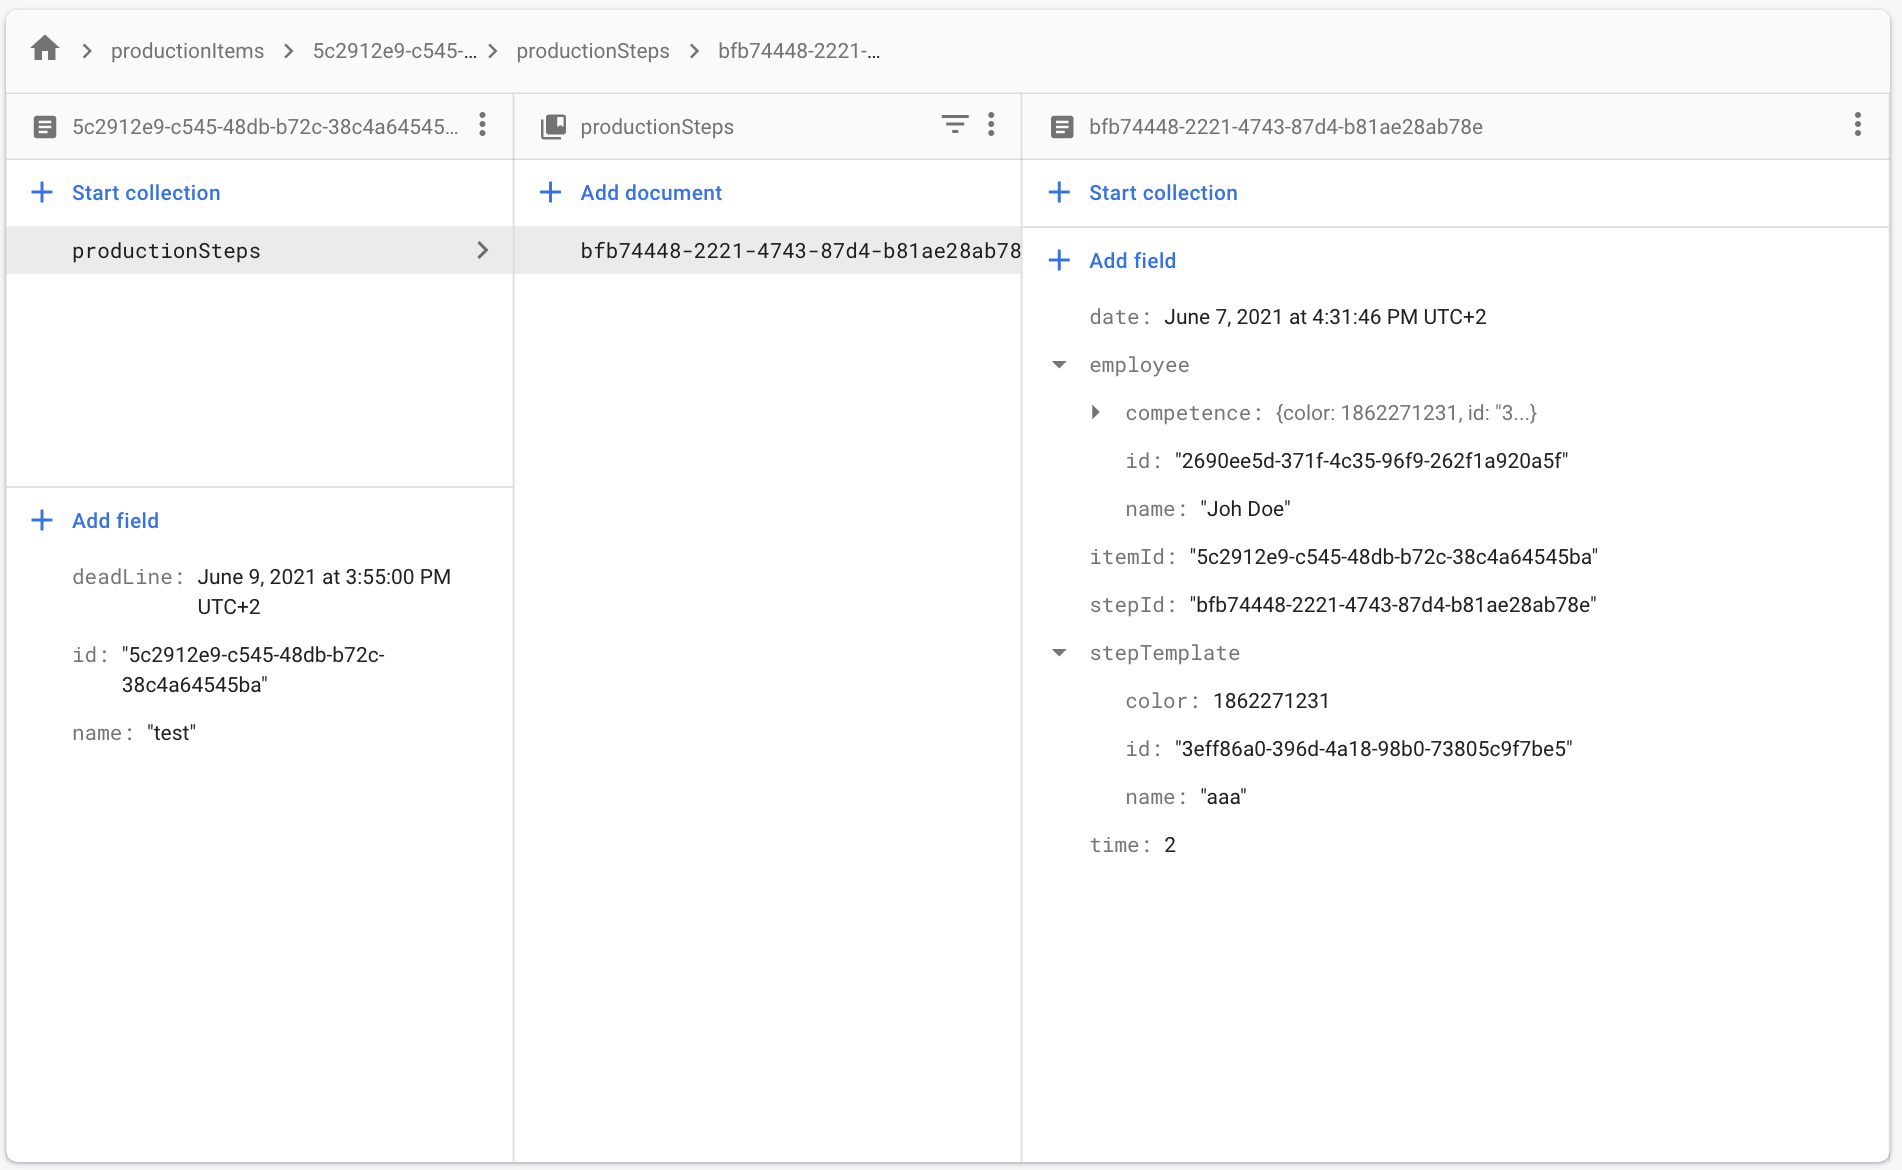
\includegraphics[scale=0.5]{img/screen_firebase2.png}
    \caption{Capture d'écran de la base de données NoSQL au 4 juin 2021}
    \label{fig:CaptureFirebase}
\end{figure}

Firebase étant une base de données NoSQL avec un stockage sous format de document\footnote{Documents JSON pour être plus précis.}, il est ainsi très facile d'accéder à n'importe quelle propriété d'un document particulier, et cela même si le document est lui-même stocké au sein d'une collection.(cf. Fig. \ref{fig:CaptureFirebase})

\clearpage
Nous avons opté pour le design de classe suivant : 

\begin{figure}[!h]
    \centering
    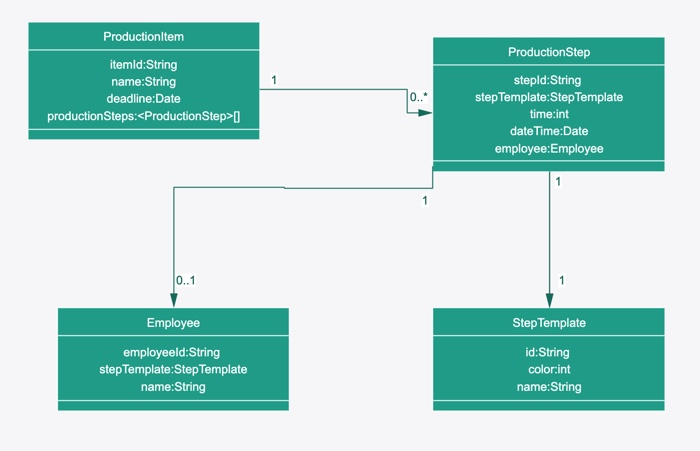
\includegraphics[scale=0.6]{img/class_diag.jpeg}
    \caption{Design de la base de données}
    \label{fig:diagClass}
\end{figure}

